\chapter{Breast Augmentation}

\section*{Overview}
Breast augmentation surgery changes breast size or shape. It may use saline-filled or silicone gel-filled implants placed under the breast tissue or chest muscle. Some people have breast volume added using their own transferred fat; fat transfer is a different procedure with different risks. This chapter focuses on implant surgery.

Implants are medical devices, not lifetime devices. A person may need another operation later to treat a complication, remove or replace an implant, or change the result. The decision should include discussion of the person's goals, alternatives, risks, costs, and long-term follow-up.


\begin{center}
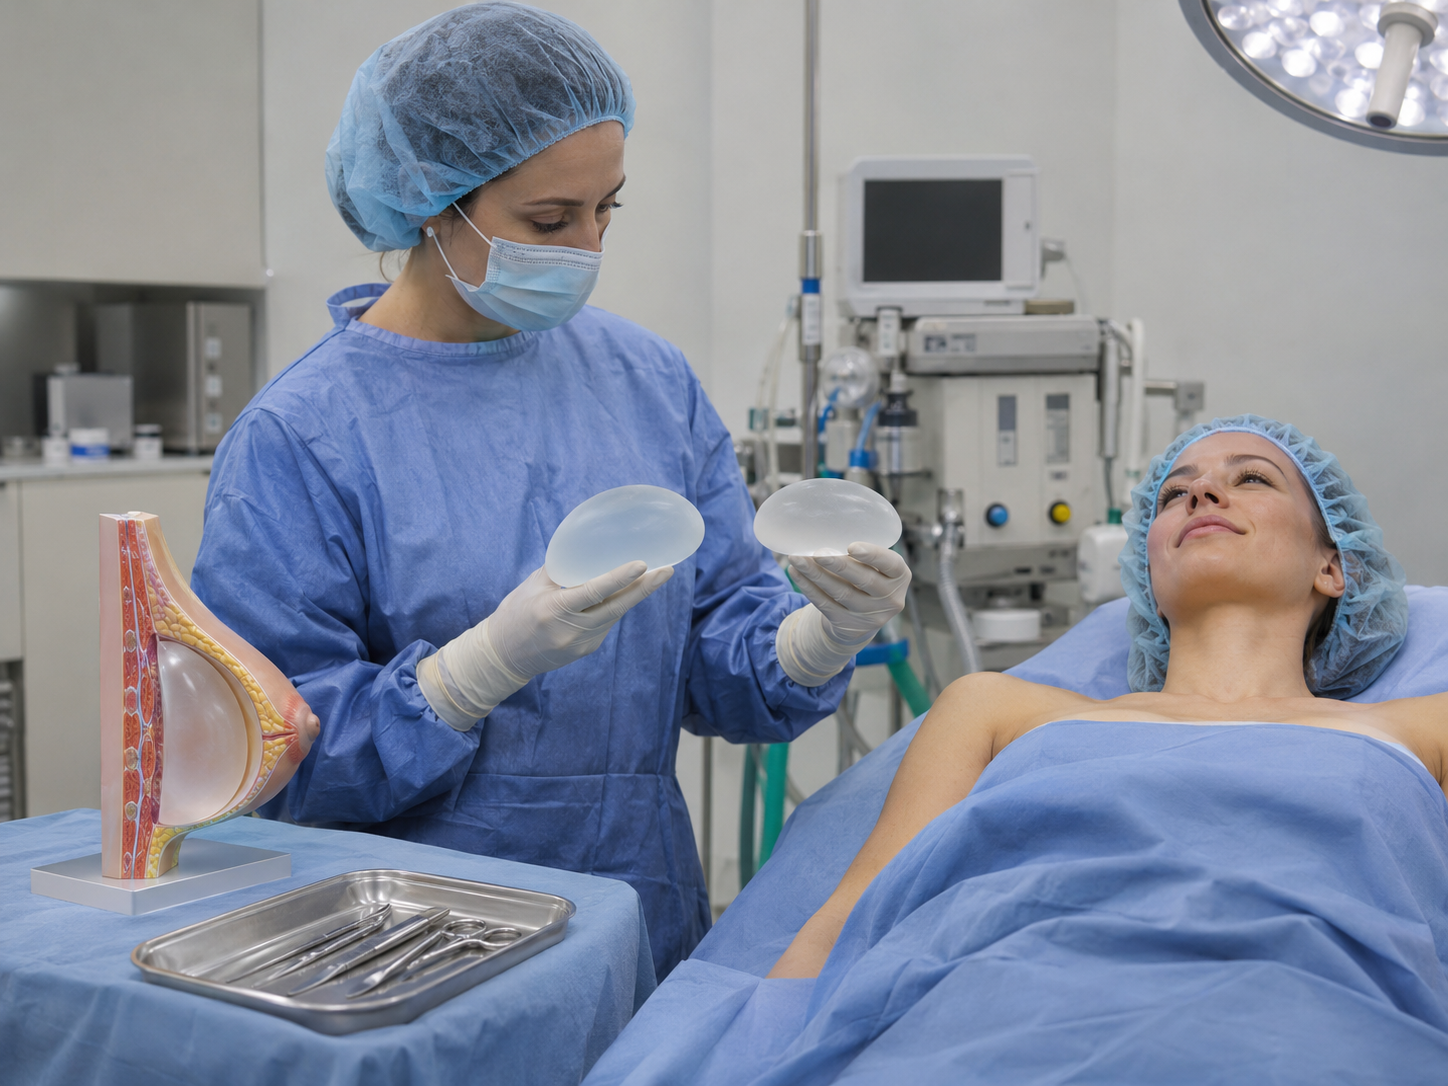
\includegraphics[width=0.82\textwidth]{images/chapters/procedure_breast_augmentation_overview.png}
\captionof{figure}{Conceptual overview of Breast Augmentation. Not a procedural guide.}
\end{center}
\section*{Alternative Names}
Augmentation mammoplasty; breast implant surgery; breast enlargement surgery.

\section*{How Implants Work}
A saline implant has a silicone outer shell filled with sterile saltwater; a silicone gel implant has a silicone shell filled with a thicker gel. Either type adds volume beneath breast tissue or the chest muscle. The implant type, size, shape, surface, incision, and position are selected with the surgeon based on anatomy, goals, and the product's approved labeling. Implants can change the appearance of the breast but do not stop normal changes from aging, pregnancy, weight change, or gravity.

\section*{Why It Is Done}
The procedure may be chosen to increase breast size, improve asymmetry, or restore volume after pregnancy, weight loss, or other changes. Implant-based surgery may also be part of reconstruction, although reconstruction has additional considerations and is not the focus of this chapter. Breast augmentation is elective and does not guarantee a particular appearance or level of satisfaction.

\section*{Role in Treatment}
This is elective surgery, not a diagnostic test. Before deciding, the patient and surgeon review alternatives, including no surgery and, when suitable, fat transfer. The surgeon should explain the implant options and provide the patient information and decision checklist for the specific device. In the United States, approved implant labeling includes a boxed warning; patients should review it and discuss questions with the surgeon before deciding.

\section*{How It Is Performed}
The operation is usually done under general anesthesia. The surgeon makes an incision, commonly under the breast, around the areola, or in the armpit, creates a space for the implant, places the implant under breast tissue or beneath the chest muscle, and closes the incision. The exact approach depends on the implant, anatomy, and surgical plan. The operation often takes one to several hours. Many patients go home the same day, while some stay overnight.

\section*{Preparation}
The surgeon reviews medical history, medicines and supplements, allergies, prior breast surgery, smoking or nicotine use, healing risks, and pregnancy or breastfeeding plans. A breast examination and age- and risk-appropriate breast imaging may be advised before surgery. Tell the surgeon if pregnancy is possible or if there is a breast lump, nipple discharge, skin change, or infection.

Before surgery, discuss the implant's fill (saline or silicone gel), shape and surface, placement, incision, expected appearance, possibility of breastfeeding changes, and how future breast screening will be done. Review the device's patient information and decision checklist, and keep the implant identification card and operative record. Follow the surgical team's instructions about eating, drinking, and medicines; do not stop prescribed medicines unless instructed.

\section*{Contraindications and Precautions}
The surgeon may postpone or advise against surgery if there is an active infection, untreated breast cancer or precancer, an uncontrolled medical condition, or a risk that makes anesthesia or healing unsafe. U.S. breast implant labeling lists current pregnancy or nursing as reasons not to have implant surgery. Smoking or nicotine use can impair healing. In the United States, FDA-approved saline implants are labeled for breast augmentation from age 18 and silicone gel implants from age 22; age requirements and indications may differ by product and country. The treating team assesses each person's health and circumstances; a past breast cancer risk or family history should be discussed but does not by itself determine whether implants are suitable.

\section*{Risks}
Possible complications include pain, bleeding, infection, blood clots, scarring, changes in nipple or breast sensation, asymmetry, rippling, implant movement, and changes to breastfeeding. Scar tissue can tighten around an implant (capsular contracture), causing firmness, discomfort, or a change in shape. An implant can leak, rupture, or deflate; silicone gel implant rupture may be silent and not detectable by touch or routine examination. Complications can lead to additional surgery, and removal without replacement can change the appearance of the breast.

Breast implants have also been associated with breast implant-associated anaplastic large cell lymphoma (BIA-ALCL), a rare lymphoma that usually starts in fluid or scar tissue around the implant rather than in breast tissue. It can sometimes spread to nearby tissue or lymph nodes. Risk is higher with textured-surface implants than with smooth-surface implants. The FDA has received reports of squamous cell carcinoma and other lymphomas in the capsule around implants. It has also received reports of other rare tumors, including sarcomas, in people with implants. These cancers appear to be rare, and their causes and rates are not known. Some people report fatigue, joint or muscle pain, memory problems, or other symptoms they call breast implant illness. These symptoms do not define a single established disease, and their causes are still being studied; some people report improvement after implant removal.

\section*{Aftercare and Recovery}
After surgery, the patient is monitored while recovering from anesthesia. Soreness, swelling, and bruising are common. The surgeon provides instructions for incision care, support garments, pain relief, activity, and follow-up. Recovery takes several weeks, and the timing for driving, work, lifting, and exercise depends on healing and the surgeon's instructions.

\section*{Outcome and Follow-up}
Follow-up checks healing, implant position, symptoms, and the patient's concerns. Breast implants are not lifetime devices, and future removal, replacement, or other surgery may be needed. Keep a record of the implant manufacturer and model and tell health care professionals and breast-imaging staff that implants are present.

Continue regular follow-up with a health care professional for as long as the implants remain in place, even if there are no symptoms. The schedule depends on the implant, the person's health, and local guidance.

Continue recommended breast cancer screening. Implants can obscure some breast tissue on mammograms, so the imaging team may use additional views. Routine imaging to look for rupture applies to silicone gel implants because a rupture may be silent; saline implant rupture usually causes visible deflation. For silicone gel implants, the FDA recommends ultrasound or MRI beginning 5 to 6 years after placement and every 2 to 3 years after that; imaging may be advised sooner if there are symptoms or an uncertain ultrasound. Follow the implant's labeling and clinician's advice, which may vary by device and location.

Contact a health care professional for a new breast lump, persistent swelling or pain around an implant, a change in breast shape or firmness, or a suspected rupture. Persistent swelling, a mass, or pain around an implant years after surgery needs prompt assessment for causes that can include BIA-ALCL. People without symptoms are not routinely advised by the FDA to have implants removed solely because of BIA-ALCL concern.

\section*{When to Seek Medical Care}
Contact the surgical team promptly for fever, increasing redness or warmth, worsening pain, unusual drainage, sudden swelling, or a new change in breast shape. Seek emergency care for severe breathing difficulty, chest pain, fainting, or heavy bleeding.

\section*{References}
\begin{enumerate}
  \item U.S. Food and Drug Administration (FDA). Things to Consider Before Getting Breast Implants. \url{https://www.fda.gov/medical-devices/breast-implants/things-consider-getting-breast-implants} (accessed November 23, 2026).
  \item FDA. Risks and Complications of Breast Implants. \url{https://www.fda.gov/medical-devices/breast-implants/risks-and-complications-breast-implants} (accessed November 23, 2026).
  \item FDA. Types of Breast Implants. \url{https://www.fda.gov/medical-devices/breast-implants/types-breast-implants} (accessed November 23, 2026).
  \item FDA. Questions and Answers about Breast Implant-Associated Anaplastic Large Cell Lymphoma (BIA-ALCL). \url{https://www.fda.gov/medical-devices/breast-implants/questions-and-answers-about-breast-implant-associated-anaplastic-large-cell-lymphoma-bia-alcl} (accessed November 23, 2026).
  \item National Health Service (NHS). Breast enlargement (implants). \url{https://www.nhs.uk/tests-and-treatments/cosmetic-procedures/cosmetic-surgery/breast-enlargement/} (accessed November 23, 2026).
\end{enumerate}

\clearpage
